\PassOptionsToPackage{lowtilde}{url}
\documentclass[aspectratio=43,english]{beamer} %If you want to create Polish presentation, replace 'english' with 'polish' and uncomment 3-th line, i.e., '\usepackage{polski}'
\usepackage[utf8]{inputenc}
\usepackage{polski} %Uncomment for Polish language
\usepackage{babel}
\usepackage{listings} %We want to put listings

\mode<beamer>{ 	%in 'beamer' mode
	\hypersetup{pdfpagemode=FullScreen}		%Enable Full screen mode
	\usetheme{JuanLesPins} 		%Show part title in right footer
	%\usetheme[dark]{AGH}                 		%Use dark background
	%\usetheme[dark,parttitle=leftfooter]{AGH}  	%Use dark background and show part title in left footer
}
\mode<handout>{	%in 'handout' mode
	\hypersetup{pdfpagemode=None}
	\usepackage{pgfpages}
  	\pgfpagesuselayout{4 on 1}[a4paper,border shrink=5mm,landscape]	%show 4 slides on 1 page
  	\usetheme{boxes}
  	\addheadbox{structure}{\quad\insertpart\hfill\insertsection\hfill\insertsubsection\qquad} 	%content of header
 	\addfootbox{structure}{\quad\insertauthor\hfill\insertframenumber\hfill\insertsubtitle\qquad} 	%content of footer
}

\AtBeginPart{ %At begin part: display its name
	\frame{\partpage}
}


%%%%%%%%%%% Configuration of the listings package %%%%%%%%%%%%%%%%%%%%%%%%%%
% Source: https://en.wikibooks.org/wiki/LaTeX/Source_Code_Listings#Using_the_listings_package
%%%%%%%%%%%%%%%%%%%%%%%%%%%%%%%%%%%%%%%%%%%%%%%%%%%%%%%%%%%%%%%%%%%%%%%%%%%%
\lstset{ %
  backgroundcolor=\color{white},   % choose the background color
  basicstyle=\footnotesize,        % the size of the fonts that are used for the code
  breakatwhitespace=false,         % sets if automatic breaks should only happen at whitespace
  breaklines=true,                 % sets automatic line breaking
  captionpos=b,                    % sets the caption-position to bottom
  commentstyle=\color{green},      % comment style
  deletekeywords={...},            % if you want to delete keywords from the given language
  escapeinside={\%*}{*)},          % if you want to add LaTeX within your code
  extendedchars=true,              % lets you use non-ASCII characters; for 8-bits encodings only, does not work with UTF-8
  frame=single,	                   % adds a frame around the code
  keepspaces=true,                 % keeps spaces in text, useful for keeping indentation of code (possibly needs columns=flexible)
  keywordstyle=\color{blue},       % keyword style
  morekeywords={*,...},            % if you want to add more keywords to the set
  numbers=left,                    % where to put the line-numbers; possible values are (none, left, right)
  numbersep=5pt,                   % how far the line-numbers are from the code
  numberstyle=\tiny\color{gray},   % the style that is used for the line-numbers
  rulecolor=\color{black},         % if not set, the frame-color may be changed on line-breaks within not-black text (e.g. comments (green here))
  showspaces=false,                % show spaces everywhere adding particular underscores; it overrides 'showstringspaces'
  showstringspaces=false,          % underline spaces within strings only
  showtabs=false,                  % show tabs within strings adding particular underscores
  stepnumber=2,                    % the step between two line-numbers. If it's 1, each line will be numbered
  stringstyle=\color{cyan},        % string literal style
  tabsize=2,	                   % sets default tabsize to 2 spaces
  title=\lstname,                  % show the filename of files included with \lstinputlisting; also try caption instead of title
                                   % needed if you want to use UTF-8 Polish chars
  literate={?}{{\k{a}}}1
           {?}{{\k{A}}}1
           {?}{{\k{e}}}1
           {?}{{\k{E}}}1
           {�}{{\'o}}1
           {�}{{\'O}}1
           {?}{{\'s}}1
           {?}{{\'S}}1
           {?}{{\l{}}}1
           {?}{{\L{}}}1
           {?}{{\.z}}1
           {?}{{\.Z}}1
           {?}{{\'z}}1
           {?}{{\'Z}}1
           {?}{{\'c}}1
           {?}{{\'C}}1
           {?}{{\'n}}1
           {?}{{\'N}}1
}
%%%%%%%%%%%%%%%%%
\setcounter{tocdepth}{1}

\newcommand\tab[1][0.5cm]{\hspace*{#1}}


\newcommand{\setcontributors}[1]{
	\let\oldmaketitle\maketitle
	\renewcommand{\maketitle}{
		\begin{frame}
			\oldmaketitle

			\noindent
				\begin{minipage}{0.4\textwidth}
						\footnotesize{\textbf{Contributors}}\\
						\scriptsize{#1}
						% \footnotesize{\textbf{Source code}}\\
						% 	\tab \scriptsize{\href{https://github.com/AGH-MOwNiT-2017/lectures}{\texttt{github.com/AGH-MOwNiT-2017/lectures}}}

				\end{minipage}
				\hfill%
				\begin{minipage}{0.45\textwidth}\raggedleft% adapt widths of minipages to your needs
					\includegraphics[width=25px, height=25px]{img/title/dice}
					\includegraphics[width=60px, height=35px]{img/title/ki}
					\includegraphics[width=30px, height=30px]{img/title/agh}

				\end{minipage}%


		\end{frame}
	}
}


\title{Metody Obliczeniowe w Nauce i Technice}
\author{Marian Bubak, Katarzyna Rycerz}
\date{}
\institute[AGH]{
	Department of Computer Science\\
	AGH University of Science and Technology\\
	Krakow, Poland\\
	\href{mailto:kzajac@agh.edu.pl}{\texttt{kzajac@agh.edu.pl}}\\
	% \href{http://www.icsr.agh.edu.pl/~mownit/}{\texttt{icsr.agh.edu.pl/$\sim$mownit}}
	\href{http://dice.cyfronet.pl/}{\texttt{dice.cyfronet.pl}}

}

%%%%%%%%%%%%%%%%
\usepackage{amsmath}
\usepackage{mathtools}
\usepackage{xfrac}
\usepackage{breqn}
\usepackage{caption}
\usepackage{enumerate}
\usepackage{comment}
%%%%%%%%%%%%%%%%
\makeatletter
\newenvironment<>{proofs}[1][\proofname]{%
	\par
	\def\insertproofname{#1\@addpunct{.}}%
	\usebeamertemplate{proof begin}#2}
{\usebeamertemplate{proof end}}
\makeatother
%%%%%%%%%%%%%%%%
\DeclareMathOperator\cas{cas}
%%%%%%%%%%%%%%%%
\newcommand*{\blockbreak}{\usebeamertemplate{block end}\usebeamertemplate{block begin}}
%%%%%%%%%%%%%%%%

\subtitle{16. Szeregi i transformaty Fouriera}
\setcontributors{Maciej Trzebiński\\Mikołaj Biel\\Rafał Stachura}


\begin{document}
	\maketitle
    %%%%%%%%%%%%%%%%
    \begin{frame}{Outline}
    	\tableofcontents
    \end{frame}

    %%%%%%%%%%%%%%%%
    \section{Wstęp}
%%%%%%%%%%%%%%%%
\begin{frame}{Wstęp}
	\textcolor{blue}{Przykładowe zastosowania transformaty Fouriera:}
	
	\begin{enumerate}[a)]
		\item metody spektralne:
		\begin{itemize}
		    \item fizyka, chemia: badanie właściwości atomów, cząsteczek, itp.
			\item na podstawie widma promieniowania elektromagnetycznego
		\end{itemize}
        \item algorytmy numeryczne:
        \begin{itemize}
        	\item równania różniczkowe
        	\item analiza: badanie jakości algorytmów (np. dla MES)
        \end{itemize}
        \item cyfrowe przetwarzanie sygnału
        \begin{itemize}
        	\item badanie składowych harmonicznych
        	\item filtracja obrazów i dźwięku
        	\item kompresja
		\end{itemize}        	
	\end{enumerate}
\end{frame}
    %%%%%%%%%%%%%%%%
	
\section{Podstawowe własności szeregów i transformat Fouriera}
%%%%%%%%%%%%%%%%
\begin{frame}[allowframebreaks]{Sposoby opisu procesu fizycznego}
	\begin{enumerate}
		\item w dziedzinie czasu (time domain) $ \implies A(t) $ \\
		$ t - \text{czas}, \quad A - \text{pewna wielkość} $
		%%%%%%%%%%%%%%%%
		\item w dziedzinie: $
		\begin{rcases*}
		\begin{array}{l}
		\text{częstości} (\omega) \\ \text{częstotliwości} (f)
		\end{array}
		\end{rcases*}$
		$\implies \widehat{A}(\omega) \quad \omega =\frac{2\pi}{T}= 2 \pi f$ gdzie $f=\frac{1}{T}$
	\end{enumerate}
	$A(t), \quad \widehat{A}(\omega) \,\, - $ dwie różne reprezentacje tego samego zjawiska związane równaniami transformat Fouriera:
	%%%%%%%%%%%%%%%%
	\begin{block}
	\centering
	\renewcommand{\arraystretch}{1.5}
	\setlength{\abovedisplayskip}{0pt}
	\setlength{\belowdisplayskip}{0pt}
	\setlength{\abovedisplayshortskip}{0pt}
	\setlength{\belowdisplayshortskip}{0pt}
	\[
	\begin{rcases*}
		A(t) = \int\limits_{-\infty}^{\infty}\frac{d \omega}{2\pi}\widehat{A}(\omega) \cdot e^{i \omega t} \\
		\widehat{A}(\omega) = \int\limits_{-\infty}^{\infty}dt \cdot A(t) \cdot e^{-i \omega t}
	\end{rcases*}
	\]
	\end{block}
	lub równoważnie:
	\begin{block}
	\centering
	\renewcommand{\arraystretch}{1.5}
	\setlength{\abovedisplayskip}{0pt}
	\setlength{\belowdisplayskip}{0pt}
	\setlength{\abovedisplayshortskip}{0pt}
	\setlength{\belowdisplayshortskip}{0pt}
	\[
	\begin{rcases*}
		A(t) = \int\limits_{-\infty}^{\infty}df \cdot \widehat{A}(f) \cdot e^{2 \pi ift} \\
		\widehat{A}(f) = \int\limits_{-\infty}^{\infty}dt \cdot A(t) \cdot e^{-2 \pi ift}
	\end{rcases*}
	\begin{array}{r}
		\rightarrow \,\, \text{korzystamy z: } \omega = 2 \pi f\\
		\text{nie trzeba pamiętać}\\ \text{o czynniku } \frac{1}{2 \pi}
	\end{array}
	\]
	\end{block}
	Trasformować można zarówno w czasie, jak i w przestrzeni,	jeśli mamy:\\
	$t - \text{czas} \rightleftharpoons \omega - \text{częstość kołowa}$
	\\ $x - \text{położenie} \rightleftharpoons k=\frac{2\pi}{\lambda}$ - liczba falowa,
	$ \lambda - \text{długość fali}$
	\\ $A(t), \quad \widehat{A}(\omega) \,\, - $ ciągłe f. swych argumentów
	\[
		A(t) \rightleftharpoons \widehat{A}(\omega) %\widehat{A}(\omega) = \Gamma[A(t)]
	\]
\end{frame}
%%%%%%%%%%%%%%%%
\begin{frame}{Definicje transformat Fouriera I}
	\begin{enumerate}[a)]
		\item FT - transformata Fouriera (Fourier Transform) \\
		$x$ - ciągłe \\
		$k$ - ciągłe \\
		$A(x), \widehat{A}(k)$ - f. ciągłe
        \begin{columns}
            \begin{column}{0.35\textwidth}
                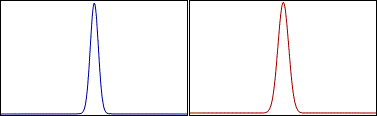
\includegraphics[width=\textwidth]{img/16/ft_wykres1.png}
            \end{column}
            \begin{column}{0.65\textwidth}
                \begin{block}
                    \centering
                    \renewcommand{\arraystretch}{1.5}
                    \setlength{\abovedisplayskip}{0pt}
                    \setlength{\belowdisplayskip}{0pt}
                    \setlength{\abovedisplayshortskip}{0pt}
                    \setlength{\belowdisplayshortskip}{0pt}
                    \[
                        \begin{array}{c}
                            \widehat{A}(k) = \int\limits_{-\infty}^{\infty}dx A(x) e^{-ikx} \\
                            A(x) = \int\limits_{-\infty}^{\infty} \frac{dk}{2 \pi} \widehat{A}(k) e^{ikx}
                        \end{array}
                        \tag{16.1}
                    \]
                \end{block}
            \end{column}
        \end{columns}
	\end{enumerate}
\end{frame}
%%%%%%%%%%%%%%%%
\begin{frame}{Definicje transformat Fouriera II}
	\begin{enumerate}[b)]
			\item W transformacie odwrotnej stosujemy - szereg Fouriera (Fourier Series) \\
		$x$ - zmienna ciągła \\
		$B(x)$ - f. okresowa ciągłej zmiennej x; okres: L
		\begin{center}
			(ciągła odcinkami wraz z pochodną: na tych odcinkach - szereg zbieżny do B(x), w punktach nieciągłości - do wartości średniej)
		
		\end{center}
        \begin{columns}
            \begin{column}{0.35\textwidth}
                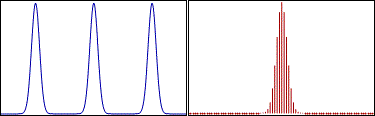
\includegraphics[width=\textwidth]{img/16/fs_wykres1.png}
            \end{column}
            \begin{column}{0.65\textwidth}
                \begin{block}
                    \centering
                    \renewcommand{\arraystretch}{1.5}
                    \setlength{\abovedisplayskip}{0pt}
                    \setlength{\belowdisplayskip}{0pt}
                    \setlength{\abovedisplayshortskip}{0pt}
                    \setlength{\belowdisplayshortskip}{0pt}
                    \[
                        \begin{array}{c}
                            \widehat{B}(k) = \int\limits_{L}dx B(x) e^{-ikx} \\
                            B(x) = \frac{1}{L}\sum\limits_{l = -\infty}^{\infty} \widehat{B}(k) e^{ikx}
                        \end{array}
                        \tag{16.2}
                    \]
                \end{block}
            \end{column}
        \end{columns}
		\begin{tabular}{ll}
			$l$ & - liczba całkowita \\
			$k$ & - dyskretne
		\end{tabular}
		\hfill $k = \underbrace{\frac{2 \pi}{L}}_{k_0} \cdot l = k_0 \cdot l$
	\end{enumerate}
\end{frame}
%%%%%%%%%%%%%%%%
\begin{frame}{Definicje transformat Fouriera III}
	\begin{enumerate}[c)]
		\item Discrete-time Fourier transform \\
		$x_p$ - dyskretne o skoku H \\
		$x_p = p \cdot H$ \\
		$p$ - liczba całkowita
        \begin{columns}
            \begin{column}{0.35\textwidth}
                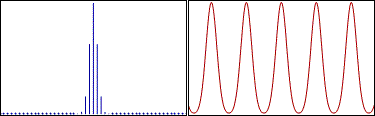
\includegraphics[width=\textwidth]{img/16/dtft_wykres1.png}
            \end{column}
            \begin{column}{0.65\textwidth}
                \begin{block}
                    \centering
                    \renewcommand{\arraystretch}{1.5}
                    \setlength{\abovedisplayskip}{0pt}
                    \setlength{\belowdisplayskip}{0pt}
                    \setlength{\abovedisplayshortskip}{0pt}
                    \setlength{\belowdisplayshortskip}{0pt}
                    \[
                        \begin{array}{c}
                            \widehat{C}(k) = H \cdot \sum\limits_{p = -\infty}^{\infty} C(x_p) e^{-ikx_p} \\
                            C(x_p) = \int\limits_{k_g} \frac{dk}{2 \pi} \widehat{C}(k) e^{ikx_p}
                        \end{array}
                        \tag{16.3}
                    \]
                \end{block}
            \end{column}
        \end{columns}
		$k$ - ciągła \\
		$\widehat{C}(k)$ - periodyczna \\
		okres $k_g = \frac{2 \pi}{H}$
	\end{enumerate}
\end{frame}
%%%%%%%%%%%%%%%%
\begin{frame}{Definicje transformat Fouriera IV}
	\begin{enumerate}[d)]
		\item fFT - skończona transformata Fouriera (finite FT) \\
		$x_p$ - dyskretne o skoku H \\
		$x_p = p \cdot H$ \\
		$D(x_p)$ - okresowa; okres: L \\
		$N$ - ilość punktów w okresie $D(x_p)$ \\
		$k$ - dyskretna, skok $k_0 = \frac{2 \pi}{L}; k = l \cdot k_0$ \\
		$\widehat{D}(k)$ - okresowa, okres $k_g = \frac{2 \pi}{H}$
		\begin{columns}
            \begin{column}{0.35\textwidth}
                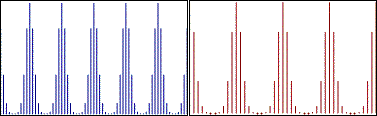
\includegraphics[width=\textwidth]{img/16/dft_wykres1.png}
            \end{column}
            \begin{column}{0.65\textwidth}
                \begin{block}
                    \centering
                    \renewcommand{\arraystretch}{1.5}
                    \setlength{\abovedisplayskip}{0pt}
                    \setlength{\belowdisplayskip}{0pt}
                    \setlength{\abovedisplayshortskip}{0pt}
                    \setlength{\belowdisplayshortskip}{0pt}
                    \[
                        \begin{array}{c}
                        \widehat{D}(k) = H \cdot \sum\limits_{p = 0}^{N-1} D(x_p) e^{-ikx_p} \\
                        D(x_p) = \frac{1}{L} \sum\limits_{l = 0}^{N-1} \widehat{D}(k) e^{ikx_p}
                        \end{array}
                        \tag{16.4}
                    \]
                \end{block}
			\end{column}
		\end{columns}
	\end{enumerate}
\end{frame}
%%%%%%%%%%%%%%%%
\begin{frame}{Związki między transformatami Fouriera}
	Przez przejścia graniczne:\\
	\centering
	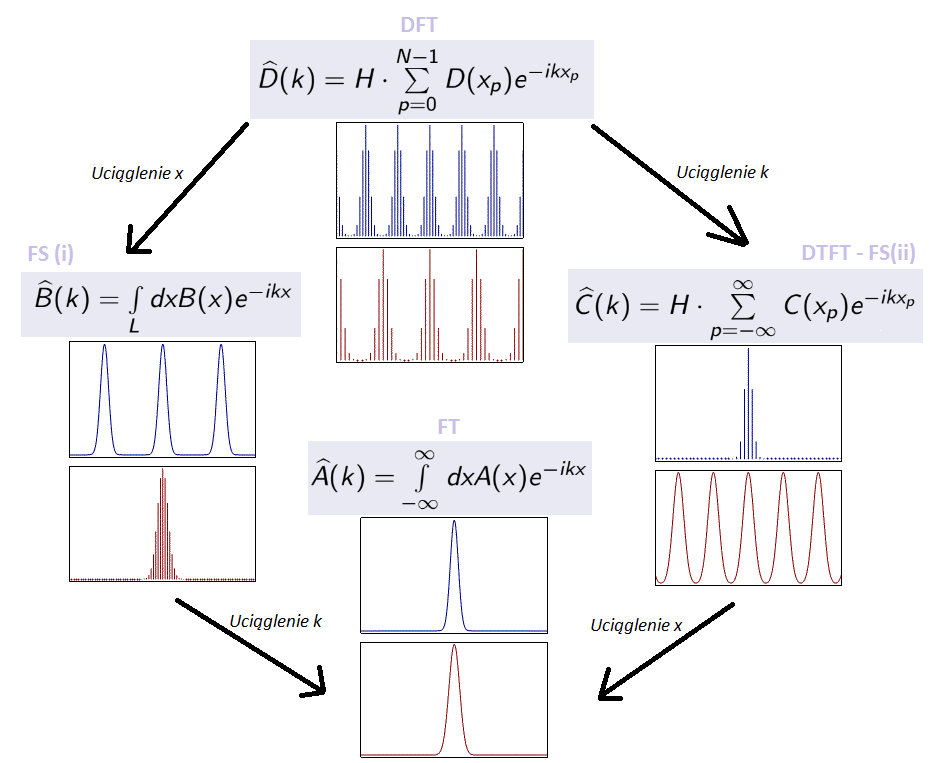
\includegraphics[height=0.8\textheight]{img/16/przejscia_graniczne.png}
\end{frame}
\begin{comment}
%%%%%%%%%%%%%%%%
\begin{frame}{Symetrie funkcji i jej transformaty I}
	Transformaty Fouriera $\to$ liniowe
	\\ Oznaczenia:
	\begin{itemize}
		\item E - even (parzysty)
		\item O - odd (nieparzysty)
		\item r - real (rzeczywisty)
		\item i - imaginary (urojony)
	\end{itemize}
	Wszystkie 4 transformaty Fouriera mają te same własności symetrii:
	\begin{align*}
		f(x) = E_r(x) + i \cdot E_i(x) + O_r(x) + i \cdot O_i(x) 
		\tag{16.5} \\
		\widehat{f}(k) = E_r(k) + i \cdot E_i(k) + i \cdot O_i(k) + O_r(k)
		\tag{16.6}
	\end{align*}
\end{frame}
%%%%%%%%%%%%%%%%
\begin{frame}{Symetrie funkcji i jej transformaty II}
	\begin{table}
		\centering
		\begin{tabular}{|c|c|}
			\hline
			$f(x)$ & $\widehat{f}(k)$ \\
			\hline
			\hline
			$r \land E$ & $r \land E$ \\
			\hline
			$r \land E$ & $i \land E$ \\
			\hline
			$i \land E$ & $i \land E$ \\
			\hline
			$i \land E$ & $r \land E$ \\
			\hline
			$r$ & hermitowska \\
			\hline
			$i$ & antyherminowska \\
			\hline
			$E$ & $E$ \\
			\hline
			$O$ & $O$ \\
			\hline
		\end{tabular}
	\end{table}
\end{frame}
%%%%%%%%%%%%%%%%
\end{comment}
\begin{frame}[allowframebreaks]{Zestawienie własności transformat}
	poza własnościami dotyczącymi pochodnej - obowiązują dla wszystkich 4 transformat \\
	$Z: f(x) \rightleftharpoons \widehat{f}(k); \quad g(x) \rightleftharpoons \widehat{g}(k)$
	\begin{block}
		\centering
		\renewcommand{\arraystretch}{1.5}
		\setlength{\abovedisplayskip}{0pt}
		\setlength{\belowdisplayskip}{0pt}
		\setlength{\abovedisplayshortskip}{0pt}
		\setlength{\belowdisplayshortskip}{0pt}
		\[
		\tag{16.7}
		\begin{array}{@{}ll}
			\text{podobieństwo:} & f(\frac{x}{a}) \rightleftharpoons |a| \cdot \widehat{f}(k \cdot a) \\
			\text{mnożenie przez stałą:} & b \cdot f \rightleftharpoons b \cdot \widehat{f} \\
			\text{suma:} & f + g \rightleftharpoons \widehat{f} + \widehat{g} \\
			\text{odwrotność:} &
			\renewcommand{\arraystretch}{1}
			\begin{array}{@{}l}
				\text{jeżeli:} \quad f(x) \rightleftharpoons \widehat{f}(k) = g(k) \\
				\text{to:} \quad g(x) \rightleftharpoons \widehat{g}(k) = 2 \pi \cdot f(-k)
			\end{array} \\
			\text{przesunięcie:} & f(x + a) \rightleftharpoons e^{ika} \cdot \widehat{f}(k) \\
			\text{pochodna:} & \frac{df}{dx} \rightleftharpoons ik \cdot \widehat{f}(k)
		\end{array}
		\]
	\end{block}
	\begin{block}{Twierdzenie o mocy}
		\[
			\int\limits_{-\infty}^{\infty} f(x) \cdot g^*(x) dx = \int\limits_{-\infty}^{\infty} \widehat{f}(k) \cdot \widehat{g}^*(k)  \frac{dk}{2 \pi}
			\tag{16.8}
		\]
	\end{block}
	Transformata zachowuje iloczyn skalarny.  \\
	Jeśli ta sama funkcja $\rightarrow$ kwadrat modułu $\rightarrow$ moc sygnału\\
	Analogicznie dla FS i fFT (wtedy sumy szeregów)
\end{frame}
%%%%%%%%%%%%%%%%
\begin{frame}{Splot (konwolucja)}
	$f(x), g(x) -$ funkcje
	$\newline$ \quad ich splot:
	\begin{block}
	\centering
	\renewcommand{\arraystretch}{1.5}
	\setlength{\abovedisplayskip}{0pt}
	\setlength{\belowdisplayskip}{0pt}
	\setlength{\abovedisplayshortskip}{0pt}
	\setlength{\belowdisplayshortskip}{0pt}
	\[
		h(x) = \int\limits_{- \infty}^{\infty} dx' f(x')g(x-x')\equiv f \ast g
		\tag{16.9}
	\]
	\end{block}
	Własności:
	\begin{table}[t]
		\centering
		\begin{tabular}{|c|l|}
			\hline
			$f \ast g = g \ast f$ & przemienny \\
			\hline
			$f \ast (g \ast h) = (f \ast g) \ast h$ & łączny \\
			\hline
			$f \ast (g +h ) = f \ast g + f \ast h$ & rozdzielny \\
			\hline
		\end{tabular}
	\end{table}
	Przykładowe zastosowanie: splot sygnału z filtrem
	\end{frame}
%%%%%%%%%%%%%%%%
\begin{frame}{Przykład operacji splotu dla dwóch wektorów kolumnowych:}
	%%%%%%%%%%%%%%%%
	$a \in I\!R^{n\times 1} \ ;\ $ $b \in I\!R^{n\times 1} \ ;\ $
	$a=\begin{bmatrix}
    		\alpha_0 \\
    		\alpha_1 \\
    		\vdots \\
   			 \alpha_{n-1}
		\end{bmatrix}$ ; \quad 
	$b=\begin{bmatrix}
    		\beta_0 \\
    		\beta_1 \\
    		\vdots \\
   			 \beta_{n-1}
		\end{bmatrix}$	
	$
		[ a * b ]_{k} = \sum_{i=0}^{k}\alpha_i \cdot \beta_{k-i};
	$\quad $a * b \in I\!R^{2n\times 1} $\quad
	
	\begin{table}[t]
		\centering
		\scalebox{0.85}{
		\begin{tabular}{ccc}
			 & $\begin{bmatrix} 
    		\beta_{n-1} \\
    		\vdots \\
    		\beta_1 \\
   			 \beta_{0}
			\end{bmatrix}$ & $\bigg\downarrow$ \\
			
			$\begin{bmatrix}
    		\alpha_0 \\
    		\alpha_1 \\
    		\vdots \\
   			 \alpha_{n-1}
			\end{bmatrix}$ &  &  \\ 
			
		\end{tabular}}
		\quad
		\scalebox{0.85}{
		\begin{tabular}{ccc}
		$\Rightarrow$&$ a * b  =$&$\begin{bmatrix} 
    											\alpha_{0} \beta_{0} \\
    											\alpha_{0} \beta_{1} + \alpha_{1} \beta_{0} \\
    											\alpha_{0} \beta_{2} + \alpha_{1} \beta_{1} + \alpha_{2} \beta_{0} \\
    											\vdots \\
    											\alpha_{n-2} \beta_{n-1} + \alpha_{n-1} \beta_{n-2} \\
    											\alpha_{n-1} \beta_{n-1} \\
   			 									0 
												\end{bmatrix}$ \\
		\end{tabular}}
	\end{table}
		\end{frame}
%%%%%%%%%%%%%%%%
\begin{frame}{Splot i jego transformaty}
$$h(x)=f(x)\ast g(x) \leftrightarrow
\widehat{h(k)}=\widehat{f(k)} \cdot \widehat{g(k)}$$
$$h(x)=f(x)\cdot g(x) \leftrightarrow
\widehat{h(k)}=\widehat{f(k)} \ast \widehat{g(k)}$$
	\begin{table}[t]
	\scriptsize
	\centering
%	\captionsetup{belowskip=-10pt,aboveskip=-10pt}
%	\caption{Splot i jego transformaty }
		\begin{tabular}{l|l|l}
			& x & k \\
			\hline
				FT
				&
				\begin{tabular}{@{}l}
					$\int\limits_{-\infty}^{\infty} dx' \cdot f(x') \cdot  g(x-x')$ \\
					$f(x) \cdot g(x)$
				\end{tabular}
				&
				\begin{tabular}{@{}l}
					$\widehat{f}(k) \cdot \widehat{g}(k)$ \\
					$\int\limits_{-\infty}^{\infty} \frac{dk'}{2 \pi} \cdot \widehat{f}(k') \cdot \widehat{g}(k - k')$
				\end{tabular} \\
			\hline
				FS(i)
				&
				\begin{tabular}{@{}l}
					$\int\limits_{L} dx' \cdot f(x') \cdot g(x - x')$ \\
					$f(x) \cdot g(x)$
				\end{tabular}
				&
				\begin{tabular}{@{}l}
					$\widehat{f}(k) \cdot \widehat{g}(k)$ \\
					$\frac{1}{L} \cdot \sum\limits_{L' = -\infty}^{\infty} \widehat{f}(k') \cdot \widehat{g}(k - k')$
				\end{tabular} \\
			\hline
				FS(ii)
				&
				\begin{tabular}{@{}l}
					$H \cdot \sum\limits_{p' = -\infty}^{\infty}  f(x'_p) \cdot g(x_p - x'_p)$ \\
					$f(x_p) \cdot g(x_p)$
				\end{tabular}
				&
				\begin{tabular}{@{}l}
					$\widehat{f}(k) \cdot \widehat{g}(k)$ \\
					$\int\limits_{k_g} \frac{dk'}{2 \pi} \cdot  \widehat{f}(k') \cdot \widehat{g}(k - k')$
				\end{tabular} \\
			\hline
				fFT
				&
				\begin{tabular}{@{}l}
					$H \cdot \sum\limits_{p' = 0}^{\infty} f(x'_p) \cdot  g(x_p - x'_p)$ \\
					$f(x_p) \cdot g(x_p)$
				\end{tabular}
				&
				\begin{tabular}{@{}l}
					$\widehat{f}(k) \cdot \widehat{g}(k)$ \\
					$\frac{1}{l} \cdot \sum\limits_{l' = 0}^{N - 1}  \widehat{f}(k') \cdot \widehat{g}(k - k')$
				\end{tabular}
		\end{tabular}
	\end{table}
\end{frame}
%%%%%%%%%%%%%%%%
\begin{frame}{Transformaty 3-D i \dots}
	Uogólnienie z 1-D na 3-D (i więcej) - bezpośrednie:
	\begin{table}[t]
		\centering
		\renewcommand{\arraystretch}{1.35}
		\[
		\tag{16.11}
		\begin{array}{c|l}
			\text{1-D} & \text{3-D} \\
			\hline
			x & \vec{x} = (x_1, x_2, x_3) \\
			k & \vec{k} = (k_1, k_2, k_3) \\
			k\cdot x & \vec{k} \cdot \vec{x} \\
			dx & d\vec{x} \\
			\frac{d\vec{k}}{2\pi} & \frac{dk}{(2\pi)^3} \\
			L & V_b = L_1 \cdot L_2 \cdot L_3 \\
			H & V_c = H_1 \cdot H_2 \cdot H_3 \\
			& \dots
		\end{array}
		\]
		\renewcommand{\arraystretch}{1}
	\end{table}
\end{frame}

	%%%%%%%%%%%%%%%%
	\section{Interpolacja trygonometryczna}
%%%%%%%%%%%%%%%%
\begin{frame}{Interpolacja trygonometryczna}
\begin{itemize}
    \item Wielomiany algebraiczne nie są dobre do opisu zjawisk okresowych
    \item Rozwiązanie: interpolacja wielomianami opartymi o funkcje  trygonomentyczne
\end{itemize}

		 funkcje okresowe o okresie L spełniają zależność  $g(y + L) = g(y)$\\
	 funkcje  trygonometryczne: okresem jest $2\pi$, po przeskalowaniu:
	$$	x = \frac{2\pi}{L} \cdot y, f(x) = g(\frac{x \cdot L}{2\pi})$$
 okresem $g(y)$ jest $L$, okresem $f(x)$ jest $2\pi$, 
	 $$f(x+2\pi)=g(\frac{(x+2\pi) \cdot L}{2\pi})=g(\frac{x \cdot L}{2\pi}+L)=
	g(\frac{x \cdot L}{2\pi})=f(x)$$
\end{frame}
\begin{frame}{Interpolacja trygonometryczna}
	szukamy wielomianu trygonometrycznego
	\[
		t_{n-1}(x) =\sum\limits_{j = 0}^{n-1} c_j \cdot (e^{ix})^{j}= \sum\limits_{j = 0}^{n-1} c_j \cdot e^{ijx}
	\]
	gdzie (przypomnienie - wzór Eulera)
	$$
	e^{ix}=cos(x)+isin(x)
	$$
	który w \underline{n punktach $x_k \in (0, 2\pi]$} przyjmuje te same wartości, co interpolowana funkcja
	\\ $t_{n - 1}(x_k) = f(x_k), k = 0, 1, \dots, n - 1$
\end{frame}
%%%%%%%%%%%%%%%%
\begin{frame}{Interpolacja trygonometryczna}
Wielomiany trygonometryczne różnią się od algebraicznych tylko wyborem zmiennej:
	\begin{theorem}
		Zadanie interpolacji trygonometrycznej ma jednoznaczne rozwiązanie.
	\end{theorem}
	%\begin{proofs}
	%	\[
		%	\sum\limits_{j = 0}^{n-1} c_j %\cdot \underbrace{(e^{ix_k})^j}_{Z_k} = f(x_k), k = 0, 1, \dots, n-1
		%	\tag{16.13}
	%	\]
	%	$\implies$ macierz układu: macierz Vandermonde'a jest nieosobliwa, \\ jeżeli \underline{$x_k$ są różne}, i:
	%	\[
	%		\det Z = \prod_{k \neq L} (Z_k - Z_L)
	%		\tag{16.14}
	%	\]
	%\end{proofs}
		W praktyce - ważny przypadek szczególny: \\
		n węzłów równoodległych, \underline{$x_k = \frac{2\pi}{n}\cdot k$}, k = 0, 1, \dots, n - 1 \\
		\underline{funkcje $e^{ijx}$}, j = 0, 1, \dots, n - 1 tworzą \underline{układ ortogonalny} w sensie iloczynu skalarnego zdefinowanego:
		$$
			\langle f|g \rangle = \sum\limits_{k = 0}^{n-1} f(x_k) \cdot g^* (x_k), x_k = \frac{2\pi}{n} \cdot k, k = 0, 1, \dots, n-1
		$$
		\end{frame}
		\begin{frame}{Interpolacja trygonometryczna}
		A dokładniej:
		\[
			\langle e^{ijx}|e^{ilx} \rangle = \sum\limits_{k = 0}^{n - 1}e^{ijx_k}  \cdot e^{-ilx_k} = n \cdot \delta_{j,l}=
			\begin{cases}
				0 & j \neq l \\
				n & j = l
			\end{cases}
		\]
		Dla
		$$
		x_k = \frac{2\pi}{n} \cdot k, k = 0, 1, \dots, n-1
		$$
		Gdzie $\delta_{j,l}$ to delta Kroneckera
		$$
		\delta_{j,l}=\left\{\begin{array}
		{l} 0,\ j\neq l\ \ \\
		1,\ j=l\ 
        \end{array}\right. 
        \text{ dla $j,l \in \{0,1,..,n-1\}$} $$

\end{frame}
\begin{frame}{Interpolacja trygonomentryczna}
Dowód:
		\[
			\langle e^{ijx}|e^{ilx} \rangle = \sum\limits_{k = 0}^{n-1} e^{ijx_k}  \cdot e^{-ilx_k} = \sum\limits_{k = 0}^{n-1} e^{i(j - l) \frac{2\pi k}{n}}(\star)
		\]
		\underline{dla $j = l$}
		\[
			(*)= \sum\limits_{k = 0}^{n-1} e^0 = n
		\]
		\underline{dla $j \neq l$}
		\[
		(*)= \sum\limits_{k = 0}^{n-1} \underbrace{e^{\frac{i(j - l)2\pi}{n} \cdot k}}_{\substack{
				\text{-szereg geom.} \\
				\text{-n-wyrazów}
			}} = a_0\frac{1 - q^n}{1 - q} = \frac{1 - \overbrace{e^{\frac{i(j - l)2\pi}{n} \cdot n}}^{cos((j - l)2\pi)+isin((j - l)2\pi)=1}}{1 - e^{\frac{i(j -  l)2\pi}{n}}} = 0
		\]
		$a_0 = 1; q = e^{\frac{i(j -  l)2\pi}{n}}$
\end{frame}

%%%%%%%%%%%%%%%%
\begin{frame}{Interpolacja trygonometryczna}
	Jakie powinny być współczynniki wielomianu interpolacyjnego $c_j$?
	
	\begin{enumerate}[1$^\circ$]
		\item
		\begin{align*}
			\langle t_{n-1}(x)|e^{ilx} \rangle = \Bigg\langle \sum\limits_{j = 0}^{n-1} c_j \cdot e^{ijx} \Bigg|e^{ilx} \Bigg\rangle = \sum\limits_{j = 0}^{n-1} c_j \cdot n \cdot \delta_{jl} = \\ = c_l \cdot n \implies \underline{c_l = \frac{1}{n} \langle t_{n-1}(x)|e^{ilx} \rangle}
		\end{align*}
		\item
		\begin{align*}
			\langle t_{n-1}(x)|e^{ilx} \rangle= \sum\limits_{k = 0}^{n-1}  \underbrace{t_{n-1}(x_k)}_{\substack{\text{=wartości} \\  \text{funkcji}}} \cdot e^{-ilx_k} =  \sum\limits_{k = 0}^{n-1} f(x_k) \cdot e^{-ilx_k} 
		\end{align*}
	\end{enumerate}
\end{frame}
\begin{frame}{Interpolacja trygonometryczna}	
 \\
	czyli:
	\[
		\underline{c_j = \frac{1}{n} \sum\limits_{k = 0}^{n-1} f(x_k) \cdot e^{-ijx_k}, j = 0, 1, \dots, n-1}
	\]
	\begin{flushleft}
		Dwa etapy obliczeń: \\
		\underline{\textit{analiza Fouriera:}} \\
		dla danych liczb zespolonych $f(x_k), k = 0, 1,\dots, n - 1$ szukamy $c_j, j = 0, 1, \dots, n-1$ \\
		\bigskip
		\underline{\textit{synteza Fouriera:}} \\
		mając liczby $c_j, j = 0, 1, \dots, n-1$ szukamy
		\[
			f(x) = \sum\limits_{j = 0}^{n - 1} c_j \cdot e^{ij\frac{2\pi}{n} \cdot k}, k = 0, 1, \dots, n-1
		\]
	\end{flushleft}
	\end{frame}
	\begin{frame}{Interpolacja trygonometryczna}
	\begin{flushleft}
		$\implies$ obie:
		\begin{itemize}
			\item dyskretne
			\item wzajemnie odwrotne
		\end{itemize}
		\textcolor{blue}{Podsumowanie:}$\newline$
		klasyczny algorytm: $(f = A \cdot C)$
		\[ n^2
		\begin{cases}
			\text{-zespolonych mnożeń,} \\
			\text{-zespolonych dodawań,} \\
			\text{-obliczeń } e^{-i\frac{2\pi kj}{n}}
		\end{cases}
		\]
		$\newline$
		Wada $\rightarrow$ duża złożoność operacji
	\end{flushleft}	
\end{frame}
	%%%%%%%%%%%%%%%%
	\section{Szybka transformata Fouriera FFT dla $n=2^m$}
%%%%%%%%%%%%%%%%
\begin{frame}[allowframebreaks]{FFT}
	\begin{itemize}
		\item Danielson, Lanczos (1942)
		\item R.L.Garwin (IBM Yorktown Heights Researcg Center)
		\item James William Cooley, John Wilder Tukey (1962)
	\end{itemize}
	\begin{table}
		\centering
		\caption{Złożoność}
		\begin{tabular}{l|lll}
			& obliczeniowa && czasowa \\
			\hline
			klasyczna FT: & $O(N^2)$ & $\implies$ & 1.5 godziny \\
			FFT: & $O(N\log_2N)$ & $\implies$ & 0.1 sekundy 
		\end{tabular}
		\caption*{Założenia: \\
			rozmiar problemu: $N = 10^6$ \\
			CPU $\sim$ 100 MFLOPS}
	\end{table}
	\textbf{Dane:} $f(x_k), x_k = \frac{2\pi}{n} \cdot k, k = 0, 1, \dots, n-1$ \\
	\textbf{Szukamy:} $c_j = \frac{1}{n} \sum\limits_{k = 0}^{n-1} f(x_k) \cdot e^{-i\frac{2\pi k}{n} \cdot j}, j = 0, 1, \dots, n-1$ \\
	\textbf{gdy:} $a_k = \frac{1}{n} \cdot f(x_k), \omega = e^{-i\frac{2\pi}{n}}$ \\
	\textbf{to:} $\underline{c_j = \sum\limits_{k = 0}^{n-1} a_k \cdot \omega^{jk}}, j = 0, 1, \dots, n-1$ \\
	\textbf{Założenie:} ilość punktów: n = $2^m \implies$ tyleż współczynników Fouriera. \\
	\begin{block}{}
	(k - numer punktu) \\
	gdy k parzyste $k = 2 \cdot k_1$ \\
	gdy k nieparzyste $k = 2 \cdot k_1 + 1$ \\
	Dziedzina k: \\
	z dołu $\underline{k_1 = 0}$ (parzyste k)  \\
	z góry: $n-1 = 2^m - 1 \implies$ k - nieparzyste: $2k_1 + 1 = n-1 \implies k_1 = \frac{n}{2} - 1$ \\
	\textbf{Rozdzielamy wyznaczanie współczyników!!!: }
	\[
		c_j = \sum\limits_{k_1=0}^{\frac{n}{2} - 1} a_{2 k_1} \cdot (\omega^2)^{j \cdot k_1} + \sum\limits_{k_1 = 0}^{\frac{n}{2} - 1} a_{2  k_1 + 1} \cdot (\omega^2)^{j \cdot k_1} \cdot \omega^j
		\tag{16.24}
	\]
	\blockbreak
	\[
	\begin{cases}
		0 \leq k_1 \leq \frac{n}{2} - 1 \\
		0 \leq j \leq n-1
	\end{cases}
	\]
Dzielimy liczby $j$ na dwa zbiory wg zasady:
		\[
		j = \frac{n}{2} \cdot l + j_1 \text{ dla (reszta z dzielenia) } 0 \leq j_1 \leq \frac{n}{2} - 1
	\]
	Mniejsze od $\frac{n}{2}$
	\[
         l=0 \text{ dla }   0 \leq j \leq \frac{n}{2} - 1 
	\]
	Niemniejsze od $\frac{n}{2}$
	\[
	l=1 \text{ dla }  \frac{n}{2}  \leq j \leq n-1 
	\]
	
	\blockbreak
	z kolei:
	\[
		\underline{(\omega^2)^{jk_1}} = \omega^{2 \cdot [\frac{n}{2} \cdot l + j_1] \cdot k_1} = \omega^{n \cdot l \cdot k_1 + 2j_1k_1} = (e^{-\frac{2\pi i}{n}})^{(n \cdot l \cdot k_1 + 2j_1k_1)} = \underline{(\omega^2)^{j_1k_1}}
		\tag{bo $e^{-2\pi \cdot i  \cdot l  \cdot k_1}=1$}
	\]
	oraz
	\[
	\omega^{j} = \omega^{\frac{n}{2} \cdot l + j_1} = (e^{-\frac{2\pi i}{n}})^{\frac{n}{2}\cdot l} \cdot \omega^{j_1}=e^{-i \pi l} \cdot \omega^{j_1}
	\]
	Czyli
	\[
	\begin{cases}
		\omega^j=\omega^{j_{1}} \text{ dla } l=0 \text{ czyli }0 \leq j \leq \frac{n}{2} - 1\\
		\omega^j=-\omega^{j_{1}} \text{ dla } l=1 \text{ czyli } \frac{n}{2}  \leq j \leq n-1\\
	\end{cases}
	\]
 \blockbreak
	\underline{i uzyskujemy}:
	Dla $0 \leq j \leq \frac{n}{2} - 1$
	\[
		c_j = \underbrace{\sum\limits_{k_1 = 0}^{\frac{n}{2} - 1} a_{2 k_1} \cdot (\omega^2)^{j_1k_1}}_{\varphi(j_1)} + \underbrace{ \sum\limits_{k_1 = 0}^{\frac{n}{2}-1} a_{2 k_1+1} \cdot (\omega^2)^{j_1k_1}}_{\psi(j_1)} \cdot \omega^{j_1}, 0\leq j_1 \leq \frac{n}{2} - 1
	\]
	Dla $\frac{n}{2}  \leq j \leq n-1$
	\[
		c_j = \underbrace{\sum\limits_{k_1 = 0}^{\frac{n}{2} - 1} a_{2 k_1} \cdot (\omega^2)^{j_1k_1}}_{\varphi(j_1)} - \underbrace{ \sum\limits_{k_1 = 0}^{\frac{n}{2}-1} a_{2 k_1+1} \cdot (\omega^2)^{j_1k_1}}_{\psi(j_1)} \cdot \omega^{j_1}, 0\leq j_1 \leq \frac{n}{2} - 1
	\]
	\blockbreak
	Każdy z 2 członów jest transformatą Fouriera - zamiast pojedynczej transformaty w n punktach $\to$ suma 2 transformat w $\frac{n}{2}$ punktach wykorzystywanych dwa razy\\
Dla $0 \leq j \leq \frac{n}{2} - 1$
	\[
		c_j = \varphi(j_1) + \omega^{j_1} \cdot \psi(j_1) ; j_1 = 0, 1, \dots, \frac{n}{2} - 1
	\]
Dla $\frac{n}{2}  \leq j \leq n-1$	
	\[
		c_j = \varphi(j_1) - \omega^{j_1} \cdot \psi(j_1) ; j_1 = 0, 1, \dots, \frac{n}{2} - 1
	\]
	itd $\dots \to$ dokonując dalszych podziałów. \\
	złożoność obliczeniowa $\leq \underline{2 \cdot Nlog_2N}$ \\
	\end{block}
	\begin{center}
	\textbf{Zasada dziel i zwyciężaj!}
	\begin{figure}
	    \centering
	   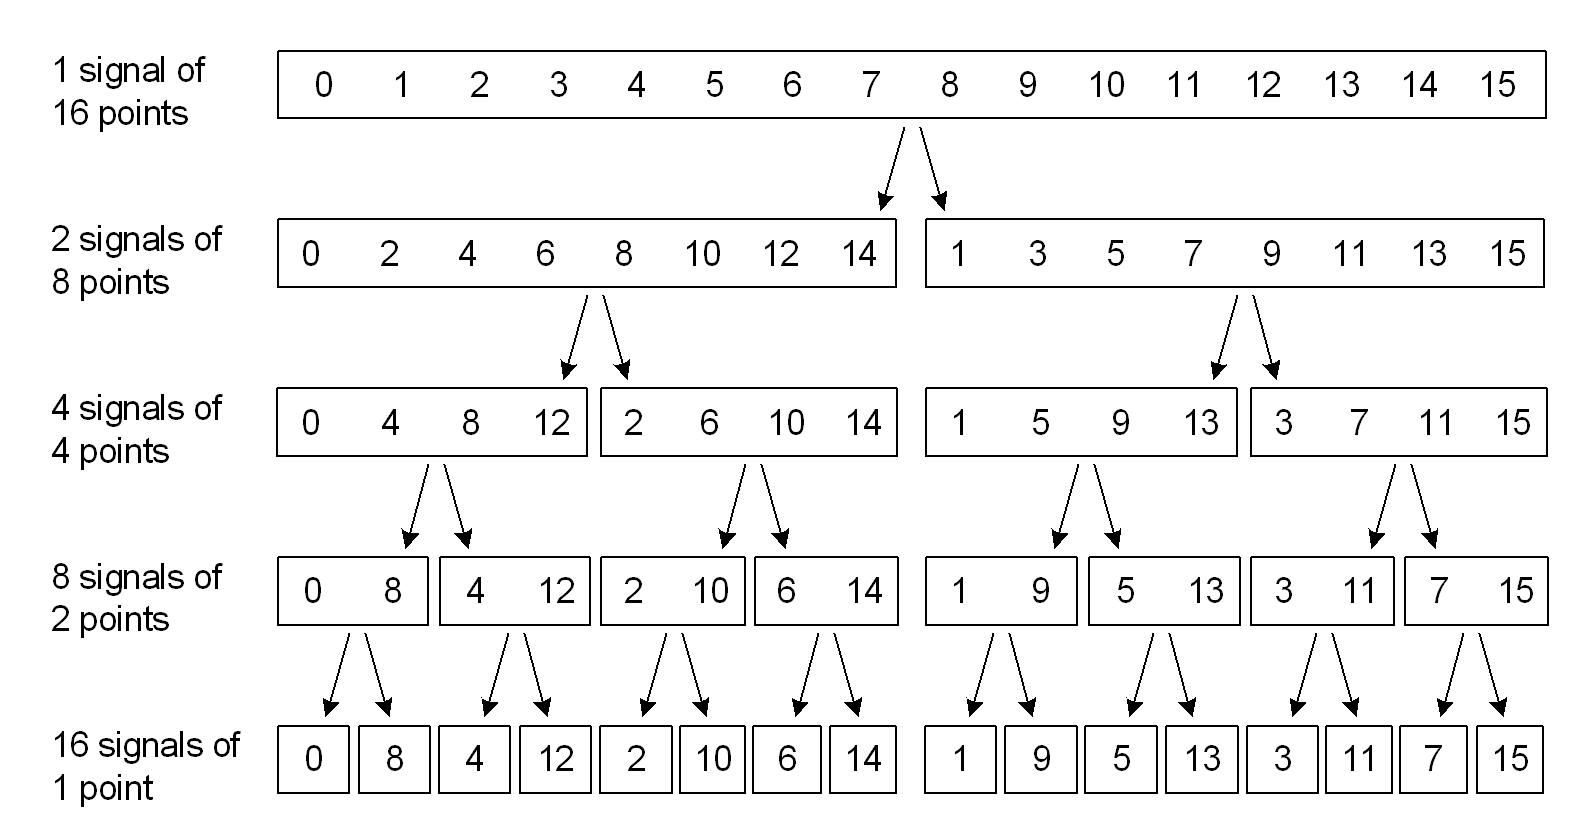
\includegraphics[width=0.8\textwidth]{img/16/podzialyFFT.png}
	    \caption{zrodlo: \url{https://riptutorial.com/algorithm/example/27088/radix-2-fft}}
	    \label{fig:my_label}
	\end{figure}
	\end{center}
	
\end{frame}  
\begin{frame}{FFT}
\begin{figure}
	    \centering
	   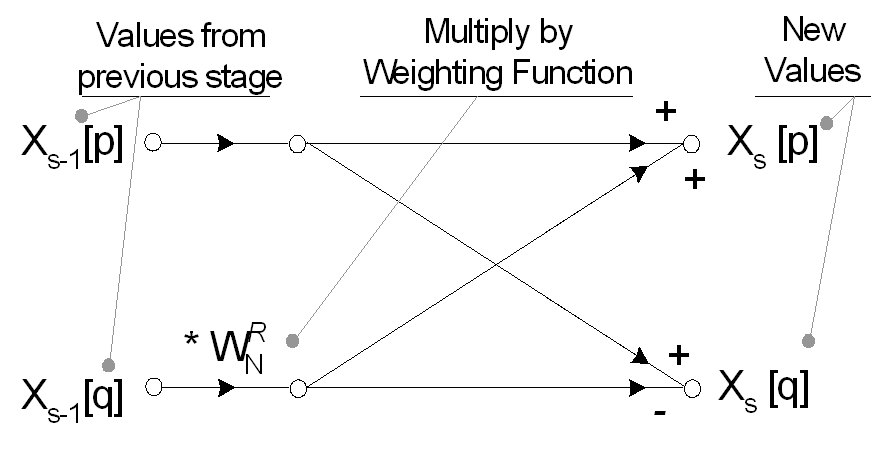
\includegraphics[width=0.9\textwidth]{img/16/bloczek_motyl.png}
	    \caption{źródlo: j.w.}
	    \label{fig:my_label}
	\end{figure}
    $W_{N}^R=(e^{\frac{-2\pi i}{N}})^R$, W naszych oznaczeniach $N=n$, $R=j_1$, $W=\omega$
\end{frame}
\begin{frame}{FFT}
    \begin{figure}
	    \centering
	   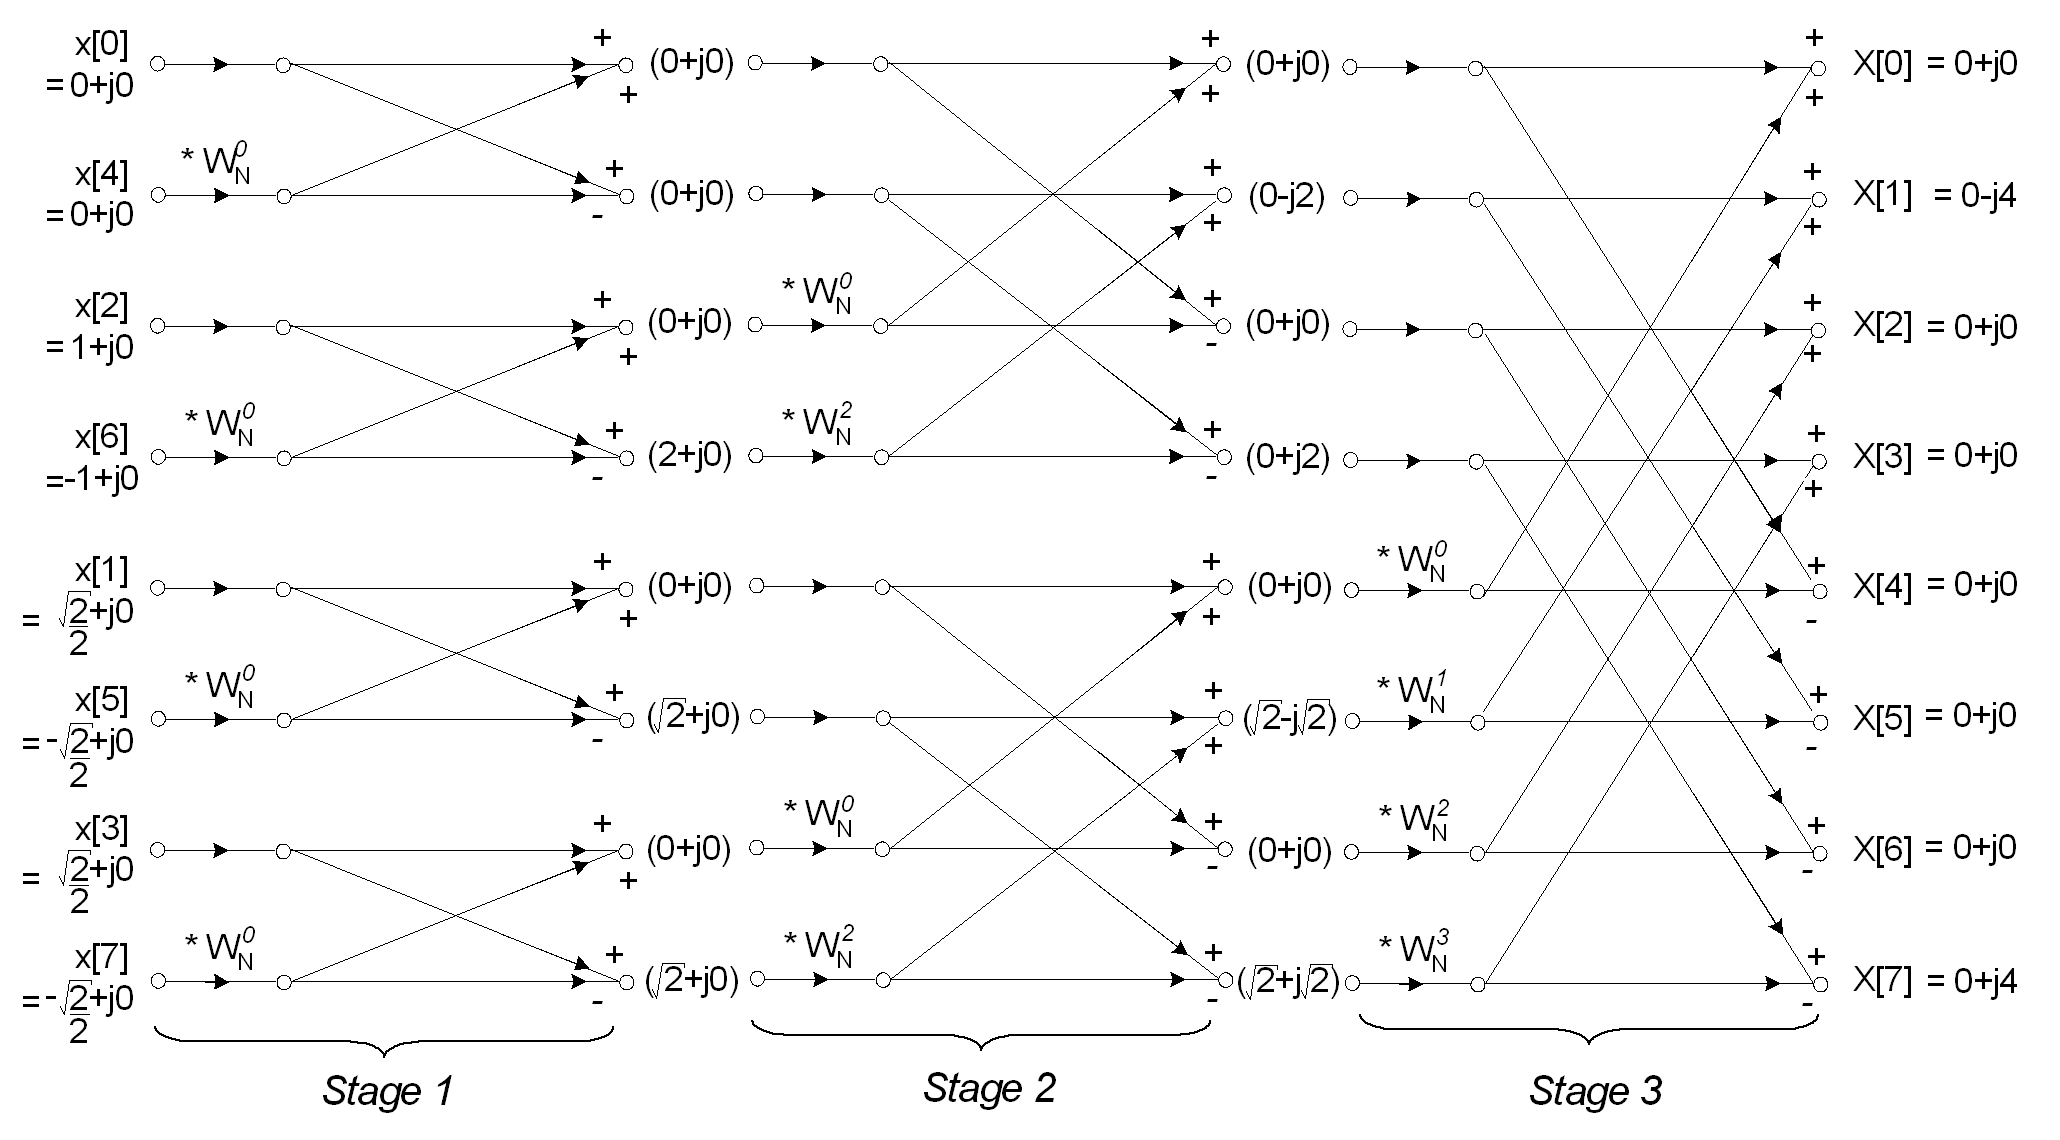
\includegraphics[width=0.8\textwidth]{img/16/motyl.png}
	    \caption{źródlo: \url{https://riptutorial.com/algorithm/example/27088/radix-2-fft}}
	    \label{fig:my_label}
	\end{figure}
\end{frame}
\begin{frame}[fragile]{Rekurencyjny algorytm FFT}
\begin{lstlisting}[language=Mathematica, mathescape]
function FFT(a)
	$n \leftarrow length[a]$
	if n = 1 
		then return a
	$\omega_n \leftarrow e^{\frac{2\pi\cdot i }{n}}$
	$\omega \leftarrow 1$
	$a_{even} \leftarrow (a_0, a_2, \dots, a_{n-2})$
	$a_{odd} \leftarrow (a_1, a_3, \dots, a_{n-1})$
	$y^{even} \leftarrow FFT(a_{even})$
	$y^{odd} \leftarrow FFT(a_{odd})$
	for j $\leftarrow$ 0 to $\frac{n}{2} -1$
		$y_j \leftarrow y^{even}_{j} + \omega y^{odd}_{j}$
		$y_{j+\frac{n}{2}} \leftarrow y^{even}_{j} - \omega y^{odd}_{j} $
		$\omega \leftarrow \omega \cdot \omega_n$
	end	
	return y
end
\end{lstlisting}

\end{frame}
	%%%%%%%%%%%%%%%%
%	\input{16_fourier/16_5_FFT_dla_przypadku_ogolnego}
	%%%%%%%%%%%%%%%%
	\section{Transformata Hartley'a}
%%%%%%%%%%%%%%%%
\begin{frame}[allowframebreaks]{Transformata Hartley'a}
	\begin{block}{Tranformata Fouriera}
	\[
		F(f) = \int\limits_{-\infty}^{\infty} X(t) e^{-i2\pi ft} dt
	\]
	\[
		X(t) = \int\limits_{-\infty}^{\infty} F(f) e^{i2\pi ft} df
	\]
	\[
		c_j = \frac{1}{n} \sum\limits_{k = 0}^{n-1} X(t_k) e^{-i2\pi j \frac{k}{n}}
	\]
	\[
		X(t_k) = \sum\limits_{k = 0}^{n-1} c_j e^{i2\pi j \frac{k}{n}}
	\]
	\end{block}
	\begin{block}{Transformata Hartley'a}
	\[
		H(f) = \int\limits_{-\infty}^{\infty} X(t) \cas(2\pi ft) dt
	\]
	\[
	X(t) = \int\limits_{-\infty}^{\infty} H(f) \cas(2\pi ft) dt
	\]
	\end{block}
	gdzie: $\cas(x) = \cos(x) + \sin(x)$\\
	istotna różnica: zamiast $\underbrace{e^{-x \cdot i}}_{\text{zespolone}}$ mamy $\underbrace{\cas(x)}_{\text{rzeczywiste}}$ ($\implies$ ilość operacji arytmetycznych i pamięć)
	\begin{block}{Wersja dyskretna HT}
	\[
		H_j = \frac{1}{n} \sum\limits_{k = 0}^{n-1} f(t_k) \cdot \cas \bigg( \frac{2\pi jk}{n} \bigg)
	\]
	\[
		f(t_k) = \sum\limits_{j=0}^{n-1} H_j \cdot \cas \bigg( \frac{2\pi jk}{n} \bigg)
	\]
	\end{block}
\end{frame}
\begin{comment}
\begin{frame}{Własności HT}
	\begin{block}{16.30}
		\centering
		\begin{enumerate}[1$^\circ$]
			\item $F_r(j) = H(j) + H(n-j)$ \\ $F_i(j) = H(j) + H(n-j)$ \\
			\item power spectrum: $P_s(j) = [H^2(j) + H^2(n-j)] \cdot \frac{1}{2}$ \\
			\item $f_1(t) \ast f_2(t) = \int\limits_{-\infty}^{\infty} f_1(\tau) \cdot f_2(t - \tau) d\tau$ \hfill - splot \\
			$f_1(t) \ast f_2(t) = F_1(f) \cdot F_2(f)$ \\
			$f_1(t) \ast f_2(t) = H_1(f) \cdot H_{2e}(f) + H_1(-f) \cdot H_{2o}(f)$
		\end{enumerate}
	\end{block}
	dla oznaczeń:
	\begin{itemize}
		\item r - real, i - imaginary \\
		\item o - odd, e - even \\
		\item F, f - Fourier, H - Hartley
	\end{itemize}
\end{frame}
\begin{frame}{Szybka Transformacja Hartley'a}
	\begin{block}{Fourier}
	\[
		F_j = F_{1j} + F_{2j} \cdot e^{-i\frac{2\pi j}{n'}} , n' = \frac{n}{2}
	\]
	\end{block}
	\begin{block}{Hartley}
	\[
		H_j = H_{1j} + H_{2j} \cdot \cos \bigg( \frac{2\pi j}{n'} \bigg) + H_2(n'-1) \cdot \sin \bigg( \frac{2\pi j}{n'} \bigg)
	\]
	\end{block}
\end{frame}
\end{comment}
\begin{frame}{Bibliografia}
	\begin{itemize}
		\item R.V.L. Hartley: A more symetrical Fourier analysis applied to transmission problems, Proc. IRE, 30 (1942) 144, \\
		\item R.N. Bracewell: The fast Hartley transform, Proc. IEEE 72 (1984) 1010 (No 8), \\
		\item M.A. O'Neill: Faster than fast Fourier, Byte, April 1988, p.293. 
	\end{itemize}
\end{frame}
\begin{frame}{FFT - przydatna w:}
	\begin{enumerate}
		\item analiza spektralna \\
		\item projektownie efektywnch algorytmów
		\begin{itemize}
			\item iloczyn wielomianów $\to$ splot 2 wektorów \\
			\item szybki binarny algorytm mnożenia liczb całkowitych
			(m. Sch\"{o}nhagego - Strassena)
		\end{itemize}
		\item $\to$ A.V. Aho, J.E. Hopcroft, J.D. Ullman: \\
		Projektowanie i analiza algorytmów komputerowych. PWN, 1983 (1974)
	\end{enumerate}
\end{frame}
	%%%%%%%%%%%%%%%%
	\input{16_fourier/16_7_transformata_fouriera_w_internecie}
	%%%%%%%%%%%%%%%%
\end{document}
